% #######################################
% ########### FILL THESE IN #############
% #######################################
\def\mytitle{Coursework Report}
\def\myauthor{Maria Luque Anguita}
\def\contact{40280156@napier.ac.uk}
\def\mymodule{Advanced Web Technologies (SET09103)}
% #######################################
% #### YOU DON'T NEED TO TOUCH BELOW ####
% #######################################
\documentclass[10pt, a4paper]{article}
\usepackage[a4paper,outer=1.5cm,inner=1.5cm,top=1.75cm,bottom=1.5cm]{geometry}
\twocolumn
\usepackage{graphicx}
\graphicspath{{./images/}}
%colour our links, remove weird boxes
\usepackage[colorlinks,linkcolor={black},citecolor={blue!80!black},urlcolor={blue!80!black}]{hyperref}
%Stop indentation on new paragraphs
\usepackage[parfill]{parskip}
%% Arial-like font
\usepackage{lmodern}
\renewcommand*\familydefault{\sfdefault}
%Napier logo top right
\usepackage{watermark}
%Lorem Ipusm dolor please don't leave any in you final report ;)
\usepackage{lipsum}
\usepackage{xcolor}
\usepackage{listings}
%give us the Capital H that we all know and love
\usepackage{float}
%tone down the line spacing after section titles
\usepackage{titlesec}
%Cool maths printing
\usepackage{amsmath}
%PseudoCode
\usepackage{algorithm2e}

\titlespacing{\subsection}{0pt}{\parskip}{-3pt}
\titlespacing{\subsubsection}{0pt}{\parskip}{-\parskip}
\titlespacing{\paragraph}{0pt}{\parskip}{\parskip}
\newcommand{\figuremacro}[5]{
    \begin{figure}[#1]
        \centering
        \includegraphics[width=#5\columnwidth]{#2}
        \caption[#3]{\textbf{#3}#4}
        \label{fig:#2}
    \end{figure}
}

\lstset{
	escapeinside={/*@}{@*/}, language=C++,
	basicstyle=\fontsize{8.5}{12}\selectfont,
	numbers=left,numbersep=2pt,xleftmargin=2pt,frame=tb,
    columns=fullflexible,showstringspaces=false,tabsize=4,
    keepspaces=true,showtabs=false,showspaces=false,
    backgroundcolor=\color{white}, morekeywords={inline,public,
    class,private,protected,struct},captionpos=t,lineskip=-0.4em,
	aboveskip=10pt, extendedchars=true, breaklines=true,
	prebreak = \raisebox{0ex}[0ex][0ex]{\ensuremath{\hookleftarrow}},
	keywordstyle=\color[rgb]{0,0,1},
	commentstyle=\color[rgb]{0.133,0.545,0.133},
	stringstyle=\color[rgb]{0.627,0.126,0.941}
}

\thiswatermark{\centering \put(336.5,-38.0){\includegraphics[scale=0.8]{logo}} }
\title{\mytitle}
\author{\myauthor\hspace{1em}\\\contact\\Edinburgh Napier University\hspace{0.5em}-\hspace{0.5em}\mymodule}
\date{}
\hypersetup{pdfauthor=\myauthor,pdftitle=\mytitle,pdfkeywords=\mykeywords}
\sloppy
% #######################################
% ########### START FROM HERE ###########
% #######################################
\begin{document}
	\maketitle
	\begin{abstract}

The aim of this coursework is to demonstrate my understanding of server-side web development and mastery of the Python Flask micro-framework by completing a personal project in which I design, implement and evaluate a web application of my choice.

My web application is called 'Eventsually' and it is an events web app. An events webpage is important because socialising reduces stress, combats loneliness and promotes people's self esteem.  There will be a higher user engagement in the events if the web page looks appealing to them and this will give people the chance to leave their houses and socialise. Dynamic designs and responsive layouts make the internet a thing of beauty.

	\end{abstract}

	\section{Introduction}

Eventsually is a web-app that let's users create an account, post events with their accounts, view other events and express interests in them, as well as message other users in order to ask for more information or any doubts about their events. Every event has its own comments to let people say what they think about them and if users want to edit or delete their account, any event they've posted or any comment, they can do so very easily too.

The web-app starts with an entertaining login page that contains TomorrowLand's 2012 official aftermovie video[1] edited to be the background, so while the user is logging in they can see how much fun it is to go to events:

    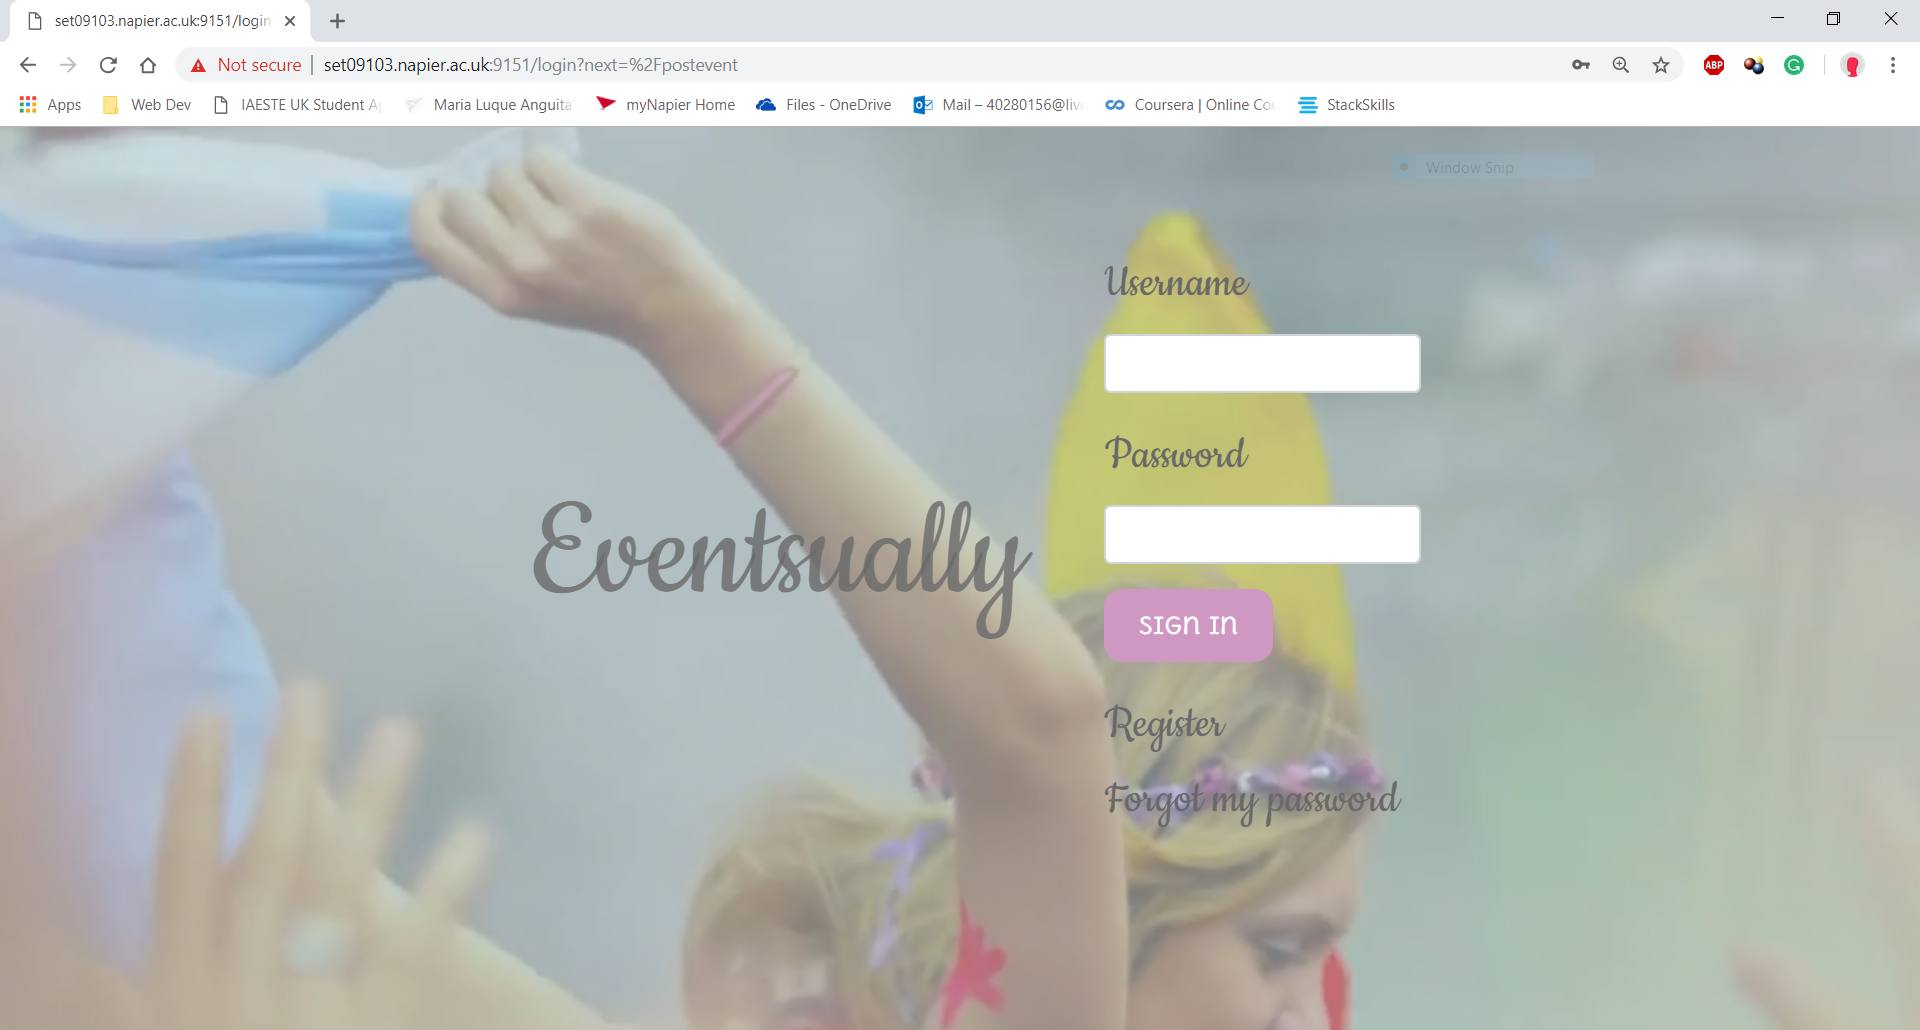
\includegraphics[width=8.5cm]{images/loginpage.jpg}

    \textbf{Figure 1 Login page}
    \vspace{2mm}

They can either Register if they are a new user, log in with their credentials or if they forgot their password they can request a new one. (In the actual web-app it won't be a static photo, it is a video that is constantly changing.)

Once the user is logged in they are redirected to the main page 'Discover Events' which displays the main events in chronological order, the events that are closer to the current day will appear first:

    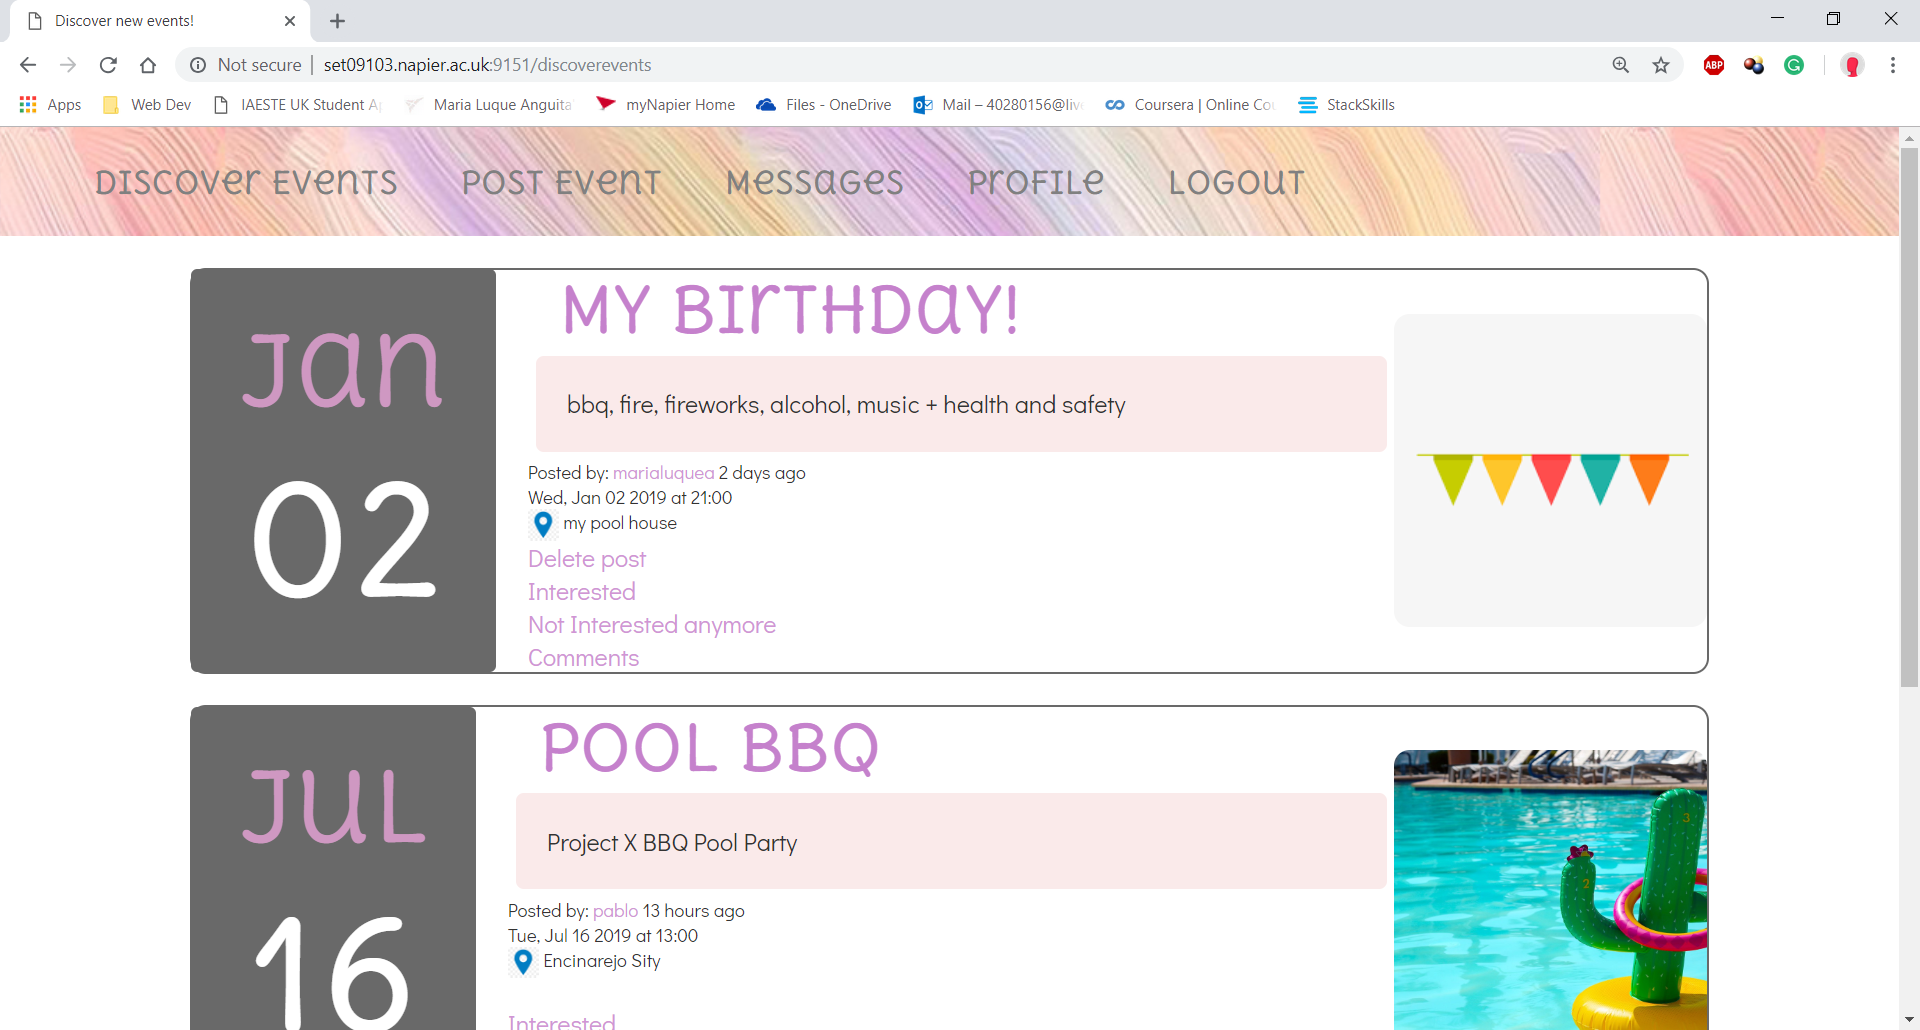
\includegraphics[width=8.5cm]{images/discover.png}

    \textbf{Figure 2 Discover Events page}
    \vspace{2mm}

The navigation bar at the top allows the user to move from one page to another without having to manually change the URL every time. However, the navigation bar only appears if the user is logged in, obviously if the user is registering or requesting another password, the navigation bar won't show, since users are not allowed to access those pages unless they are logged in.

From the navigation bar the users access their profile page, they can read their messages or they can choose to post an event. When they are done using the web-app they can log out. The 'messages' part will change depending on how many unread messages the user has. A badge next to it will appear with the number of unread messages, and once the user clicks in the Messages and reads them the badge disappears but the user can still see all the received messages (and delete them or reply to the sender).

    \section{Design}

The web-app is structured like as shown below:

    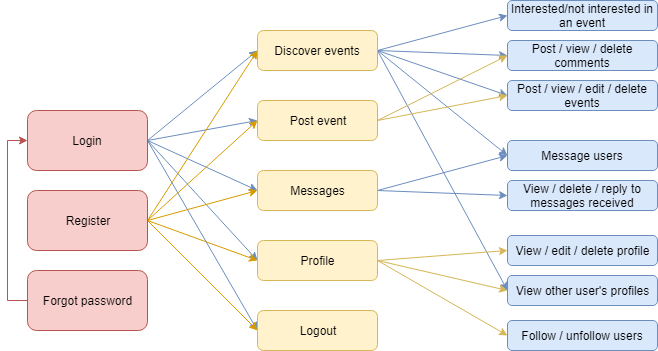
\includegraphics[width=8.5cm]{images/hierarchy.png}

    \textbf{Figure 3 How the web-app is structured}
    \vspace{2mm}

At first when the users register they are prompted to insert a password twice, to validate that the user is sure of what they are typing. The first password is saved, but only after being hashed. If an administrator accesses the database they will not be able to view anyone's password because they are all hashed using a python's hashing library 'werkzeug', which means 'tool' in German. The purpose of this is to verify the user's password with the two methods described below without having to save the actual password. If the data is compromised, it will never expose the user's password.
    \begin{lstlisting}[caption = Hashing passwords]
    from werkzeug.security import generate_password_hash, check_password_hash
    from hashlib import md5

    def set_password(self, password):
        self.password_hash = generate_password_hash(password)

    def check_password(self, password):
        return check_password_hash(self.password_hash, password)
    \end{lstlisting}

Once registered, users can access all different parts in the hierarchy. Eventsually is designed so that users can navigate easily by changing the URL or by clicking the links around the app. If they make any mistake they will be redirected to an error page that will give them the option to go back and a message will be sent to the administrators describing the errors, if it was an internal server error.

Users can follow other users and see the events they have posted and the events they have shown interest in.

    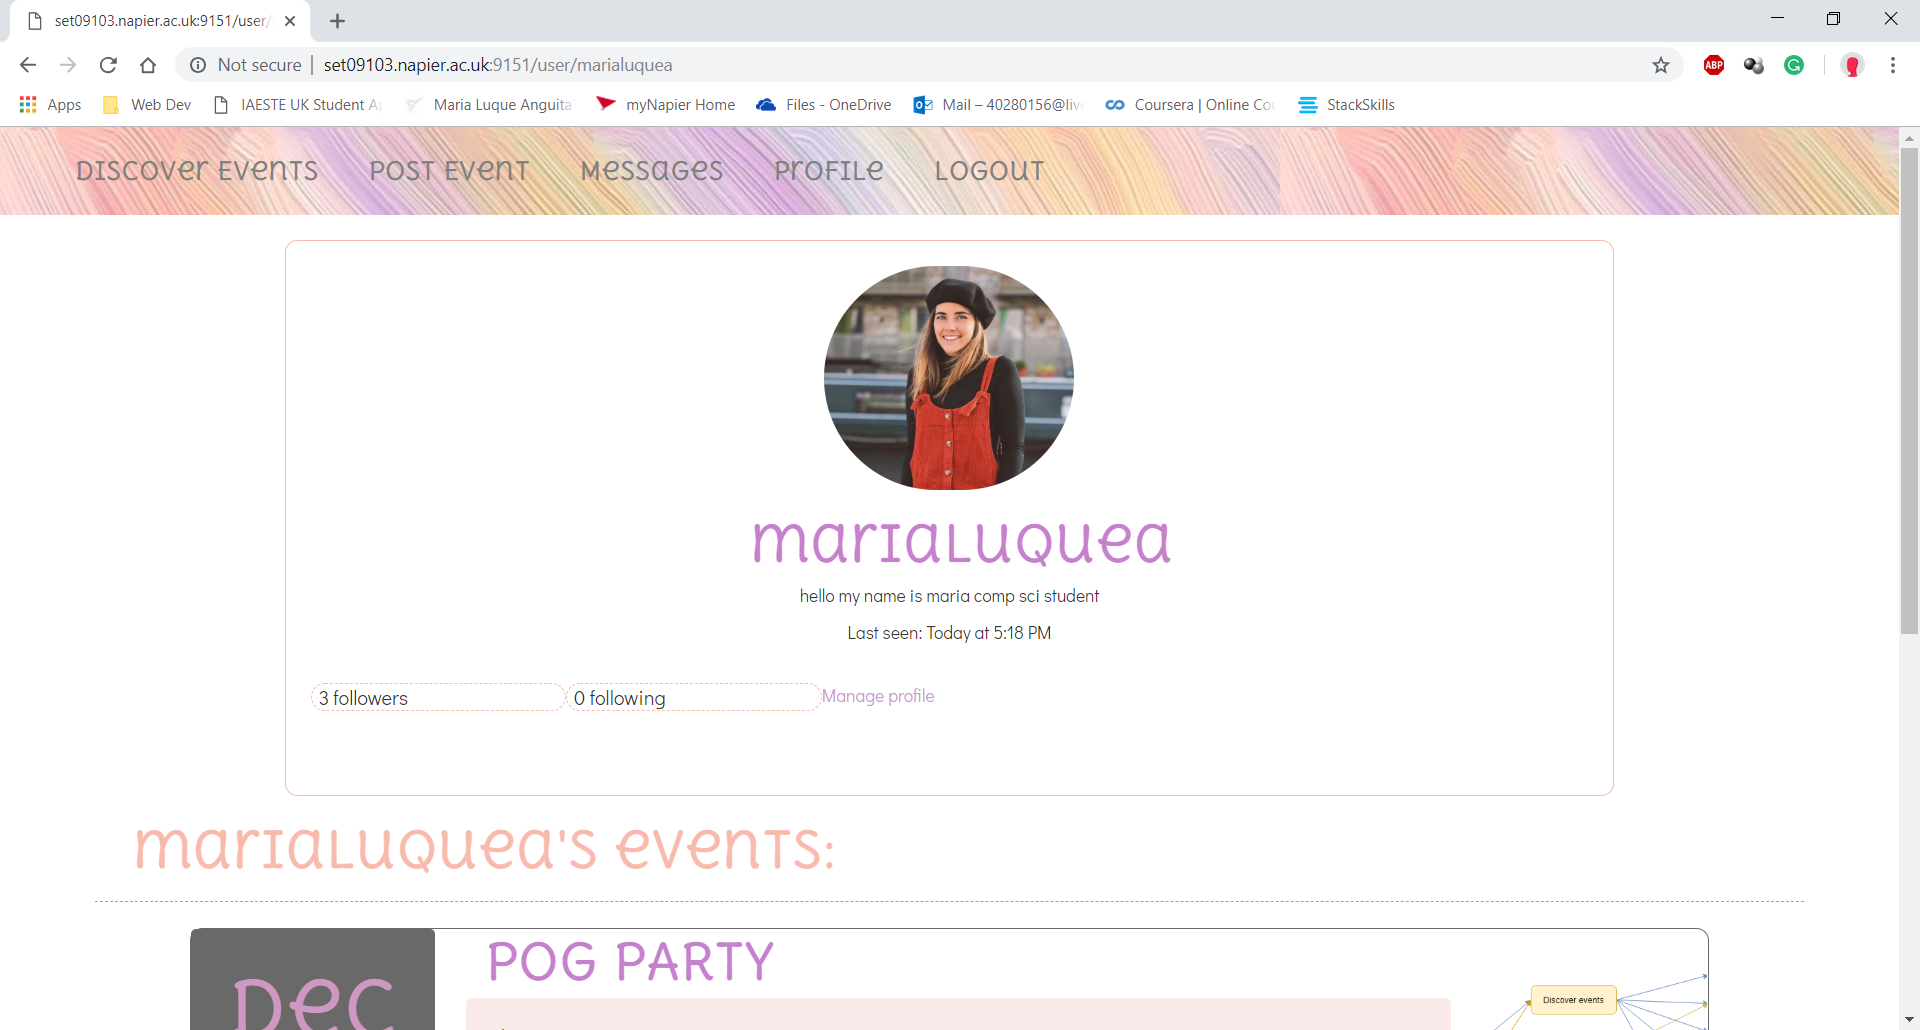
\includegraphics[width=8.5cm]{images/user.png}

    \textbf{Figure 4 User Profile page}
    \vspace{2mm}

The Follow button will be changed to Unfollow if the current user follows that person, and obviously it doesn't appear if the user is on its own profile page because users cannot follow themselves. The options to edit or delete your account will only appear if you are that user, and if you are viewing another user you will see the option to send them a message instead.

From the Discover Events page the users can view all the events and in each event, they can either show interest on them (and they will appear in their profile) or say if they are not interested anymore (will stop appearing in their profile), they can click on it to view the event, post a comment and view all the other comments, and if they are the creators of the event they can also edit it or delete it.

    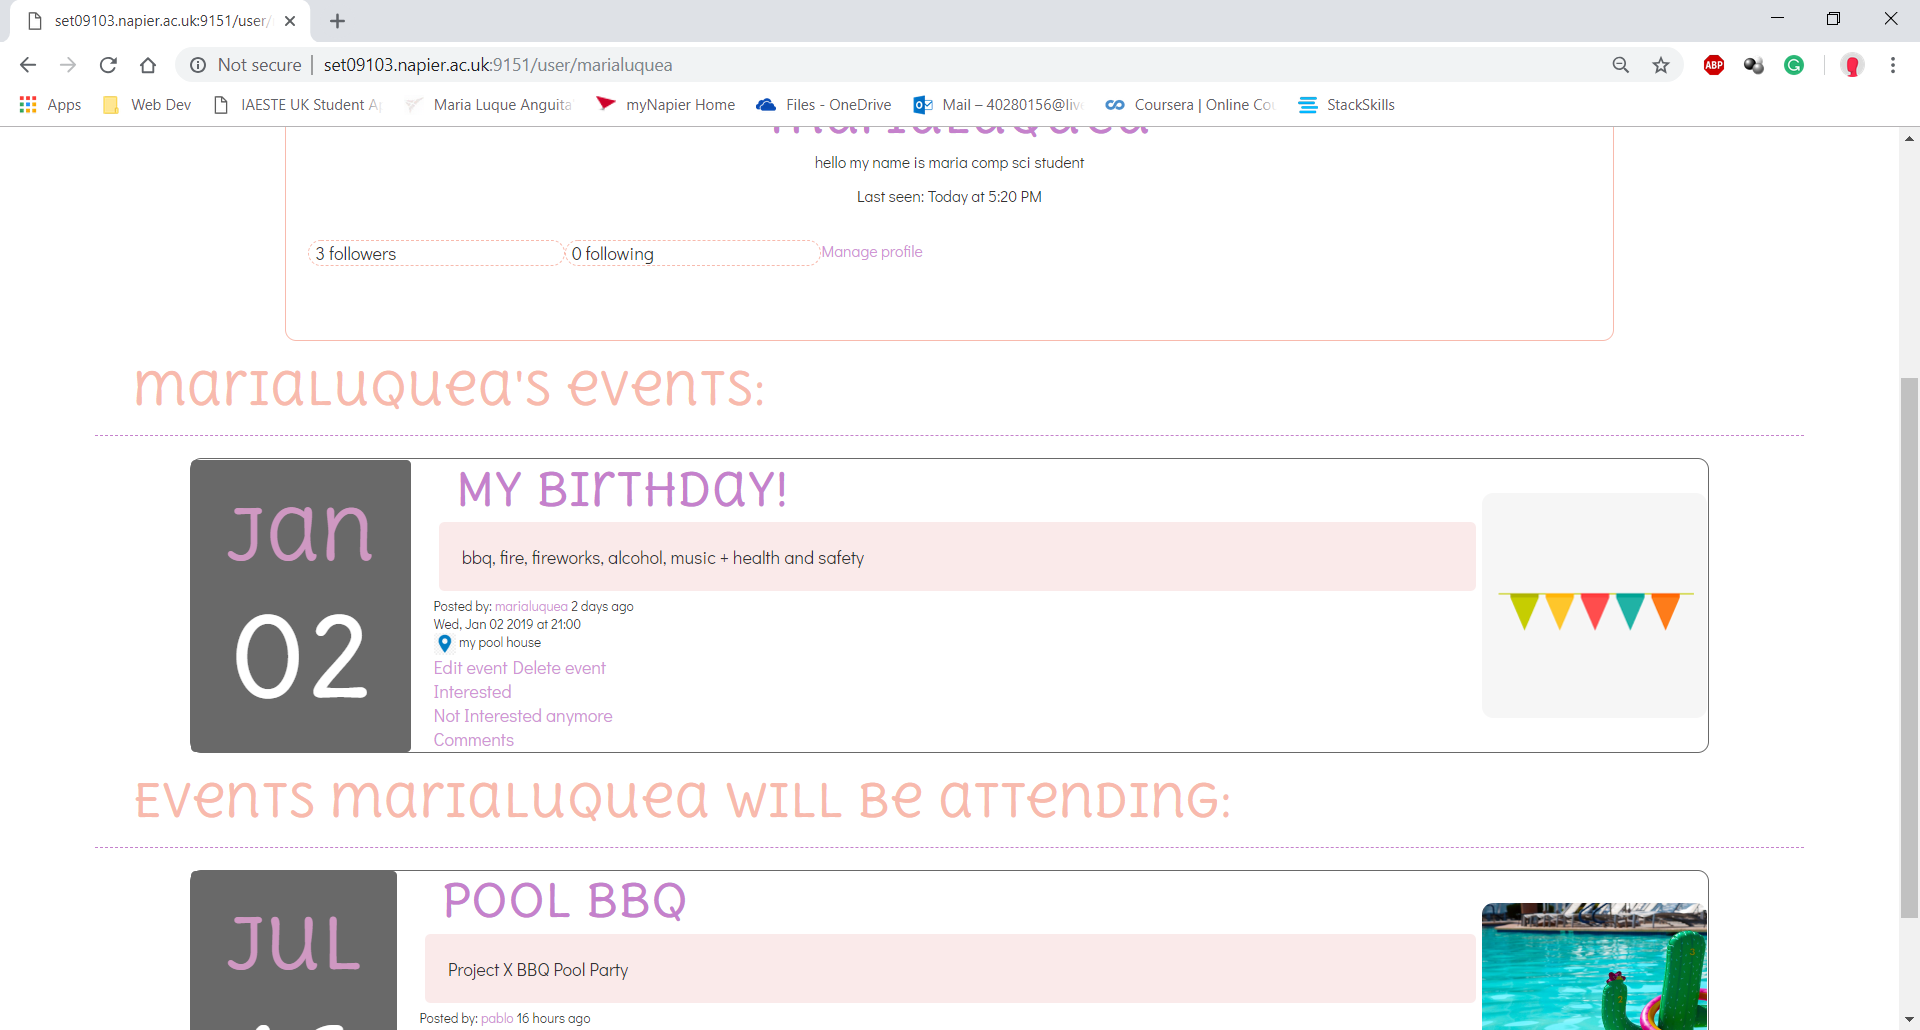
\includegraphics[width=8.5cm]{images/userevents.png}

    \textbf{Figure 5 User Profile showing user's events and the events they are interested in}
    \vspace{2mm}

    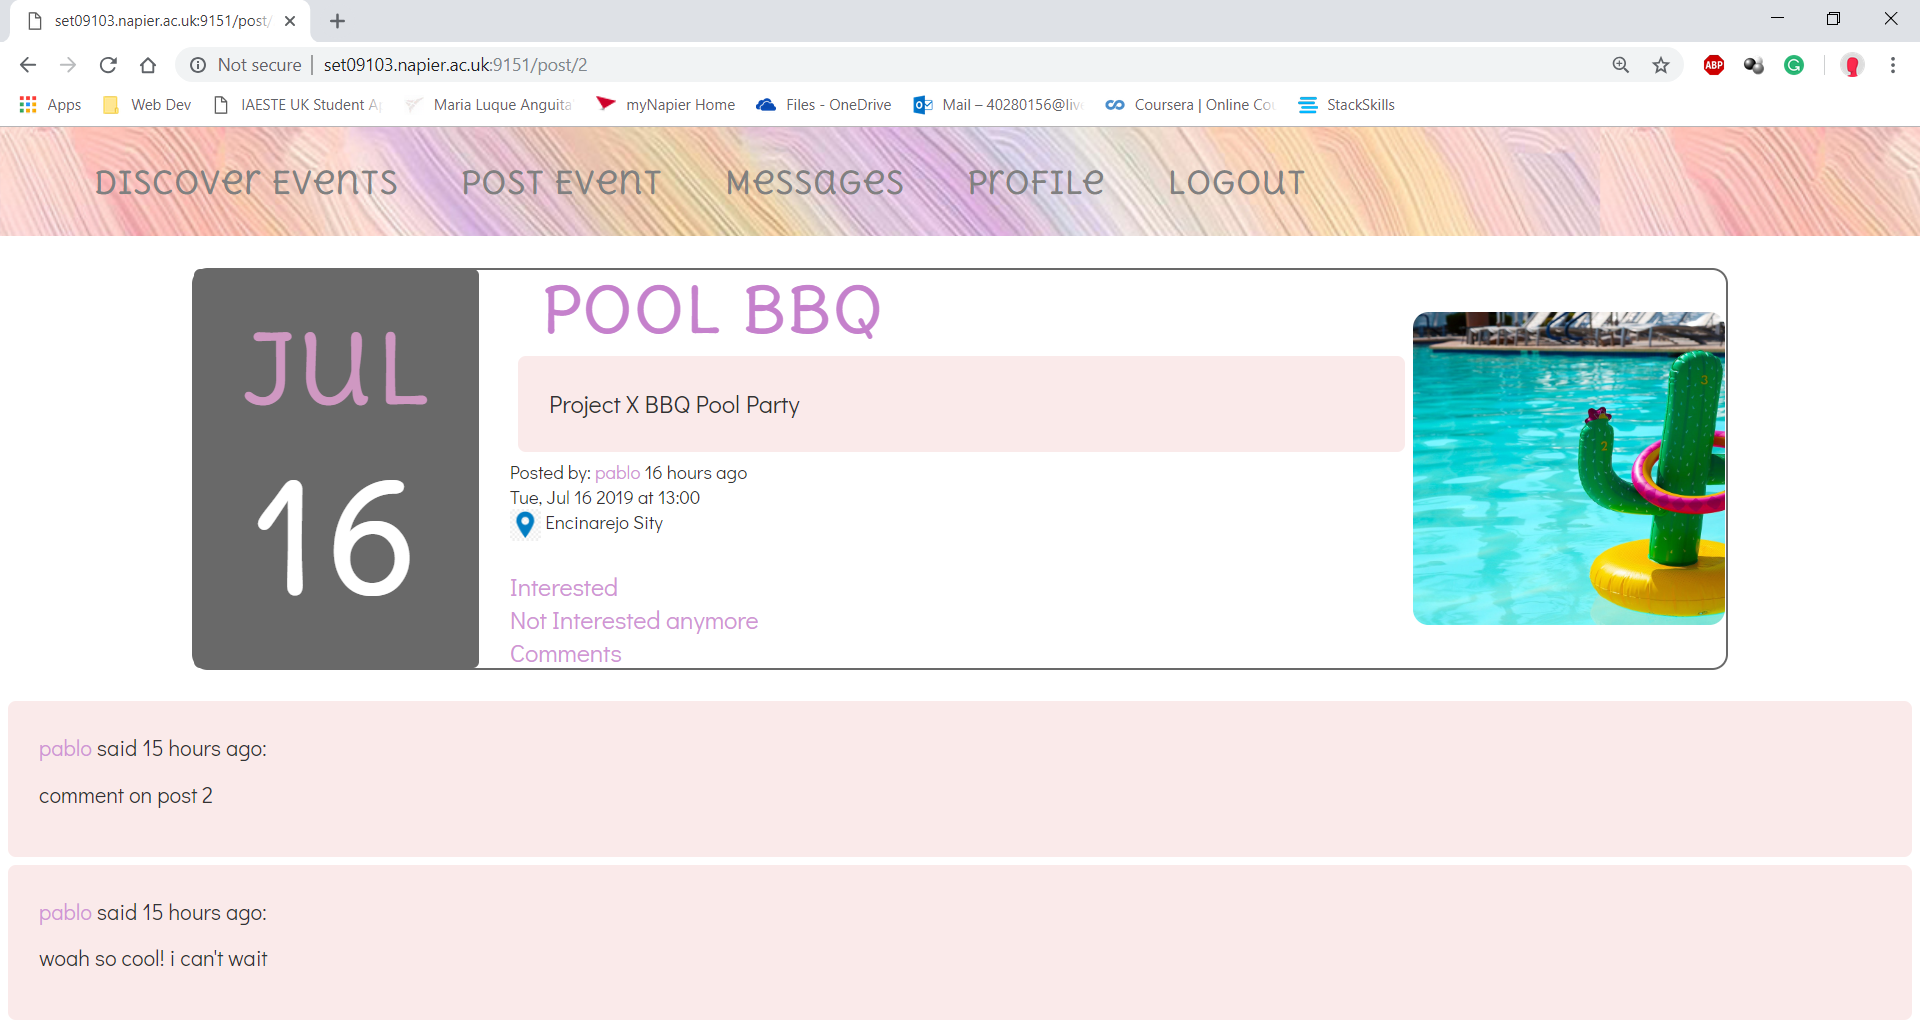
\includegraphics[width=8.5cm]{images/event.png}

    \textbf{Figure 6 Event and its comments}
    \vspace{2mm}

The option to edit the event will only appear if the current user is the creator of it and only the rest of the users can show interest in the post or not, the event creator is obviously interested. Everyone can click on 'Comment' and a form will appear under the post allowing the user to post a comment.

All of the forms in Eventsually have the same CSS to keep consistency. This inspiration came from a website[2] that had many logins designed by Digital Media people to provide inspiration for developers:

    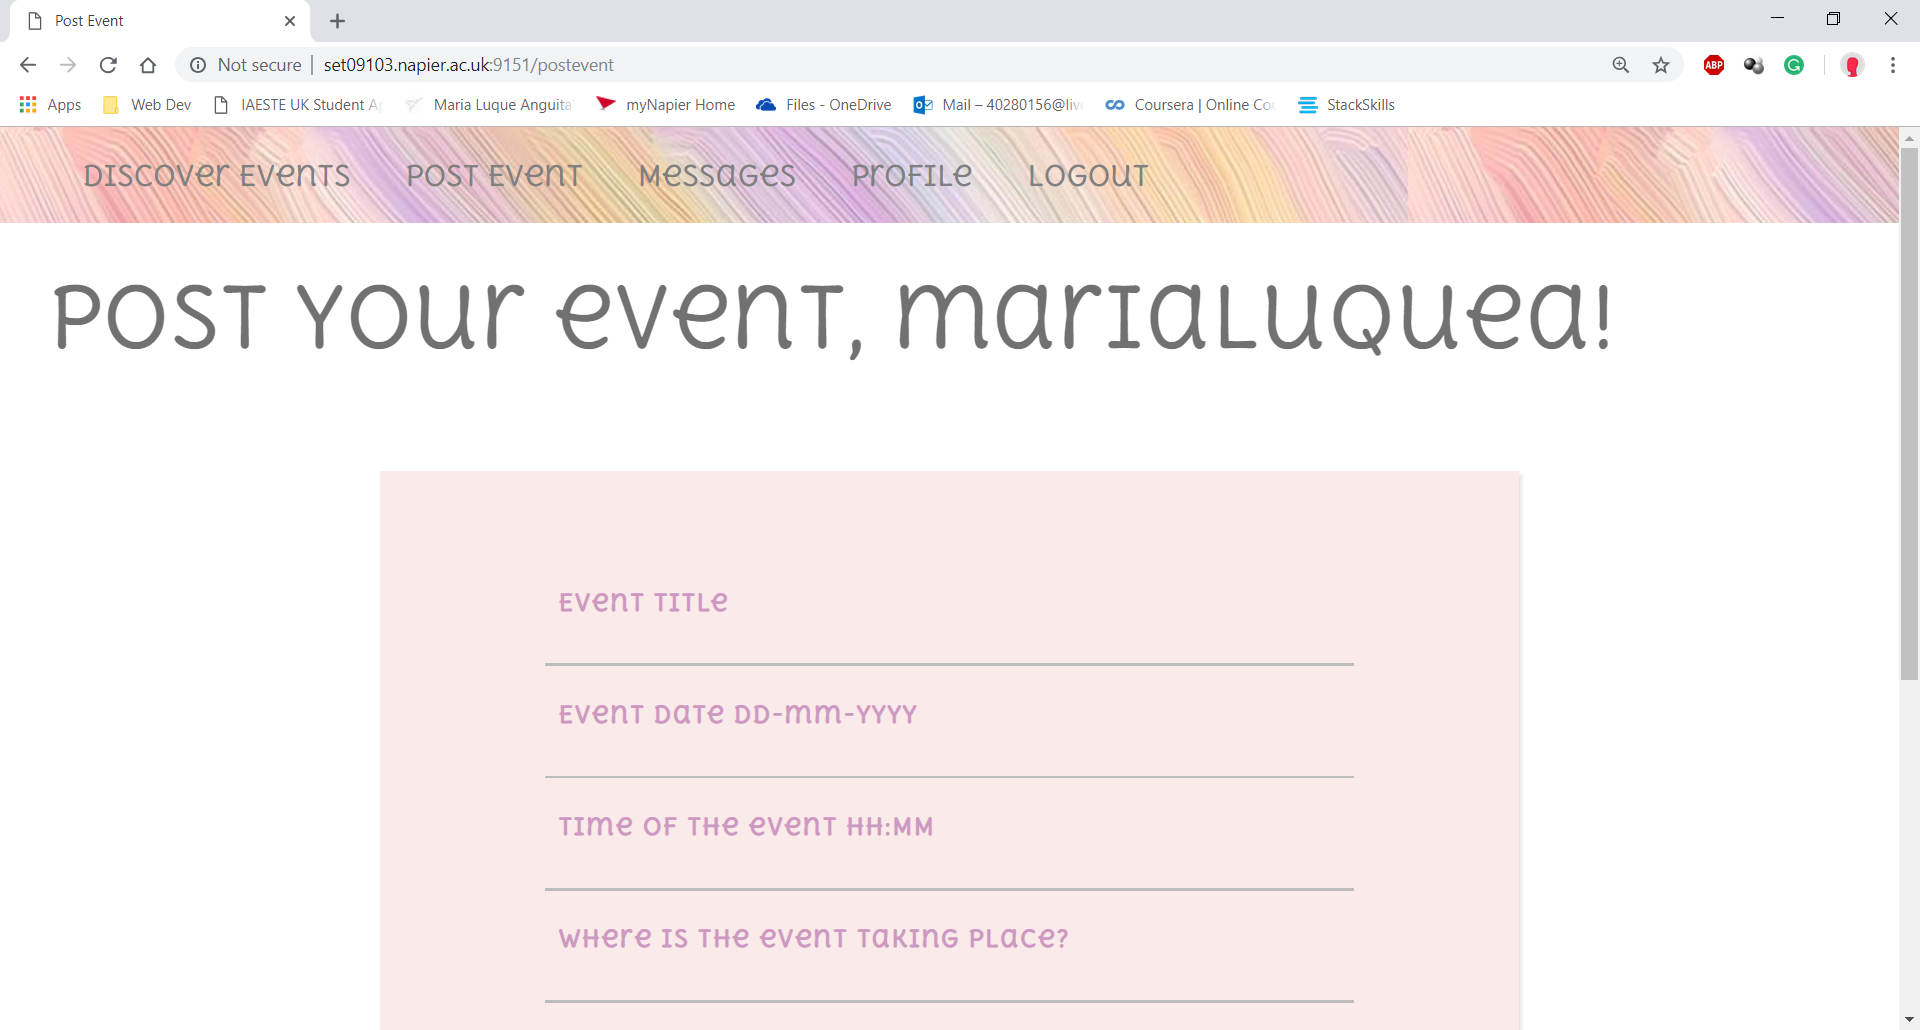
\includegraphics[width=8.5cm]{images/postevent.png}

    \textbf{Figure 7 Post Event Form}
    \vspace{2mm}

However, if the user requests a password reset the form won't show the navigation bar since they are not logged in, but there is still a form to enter the user's email. An email will then be sent to that email (only if there is an actual user with that email in the database) with a token in the URL that then allows them to enter their new password and they can log in again.

    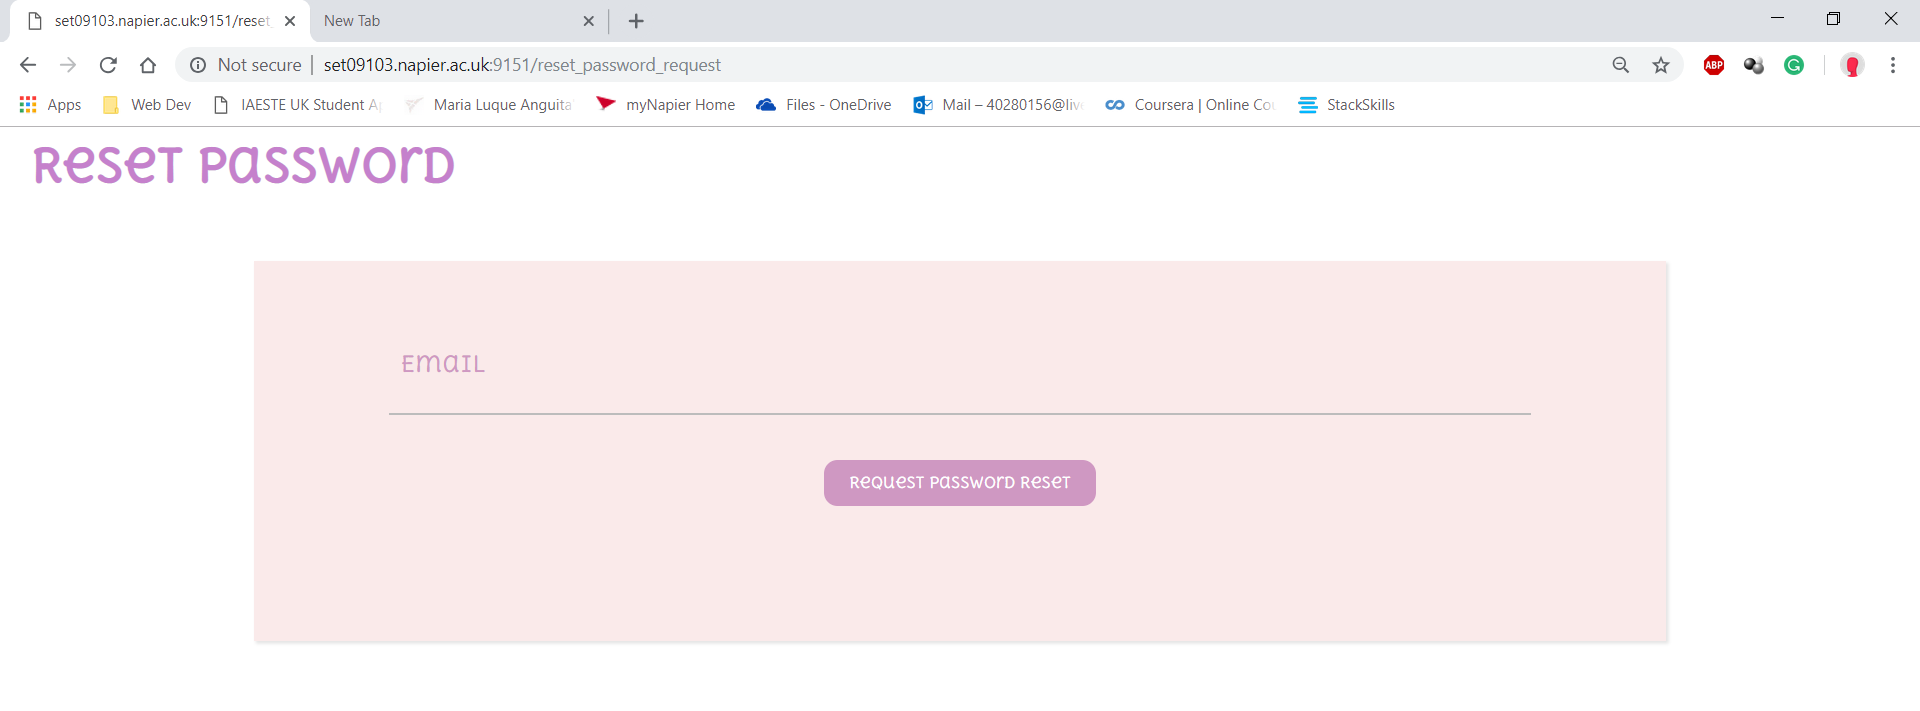
\includegraphics[width=8.5cm]{images/resetp.png}

    \textbf{Figure 8 Password reset request with no navigation bar but still same form format}
    \vspace{2mm}

The messages have the same format as the comments also to keep consistency. All of the colours in the web-app come from the navigation bar image. I used an online website that allowed me to upload an image and get the hex colour numbers from there to make sure it would all look good together. Messages also display the option to reply to the person who sent the message and the option to delete the message. They are ordered in chronological order, the most recent messages are at the top.

    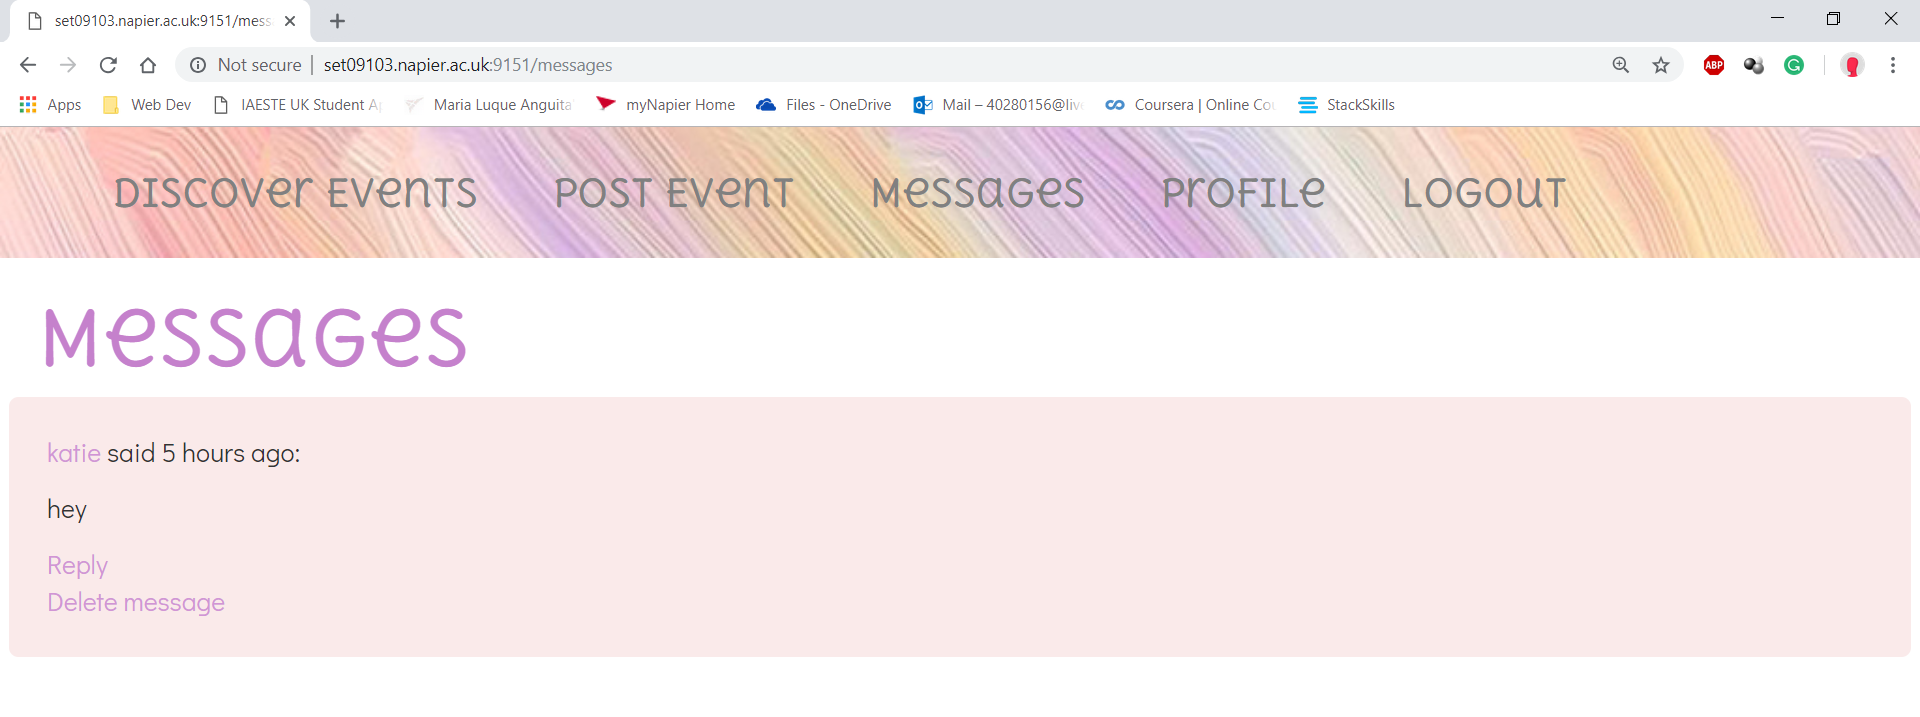
\includegraphics[width=8.5cm]{images/messages.png}

    \textbf{Figure 9 Private messages}
    \vspace{2mm}

All the information in the web-app is saved in a database using SQLAlchemy and it is programmed so that it doesn't crash. During the debugging part I had a couple of problems when querying the database for objects that didn't exist, therefore I put the queries inside try and catches and if something goes wrong, instead of crashing it will just display a message saying what went wrong but it won't stop the user from doing what they want to do.

At first I chose to use PeeWee instead of SQLAlchemy for my database because I read the documentation and watched some video tutorials and it looked like a very well maintained alternative to SQL. However, more people use SQL so whenever I encountered a problem it was easier to find a solution for SQL than PeeWee.

    \section{Enhancements}

In the next months, I will be improving my web-app and adding new features that will make it more usable. Some of the ideas I thought for improvements came from my research on how to analyse and enhance a website[3].

First of all it would be useful for users to see the events in a map so they can see where the closest events are and hopefully if enough users were to use the website you could select an options that only shows events on that day or that week or whenever.

I could also add a payments functionality so that if the event requires tickets, the users can buy them directly from the website and not from the link given in the event post.

Comments to comments would be useful, as well as having a search for all the page or event categories so the users can search for event categories, also email alerts every time an event that you are interested in changes so the user doesn't miss any detail.

    \section{Critical Evaluation}
For this part of the report, I base my critical evaluation in a published article on how to evaluate web pages[4] and my personal assessment.

Passwords should never be stored in their original version, they should be hashed to prevent risks, I have implemented that in Eventsually, as well as making the code efficient: there are no repeated loops. If anything was to be done more than once, I created a separate function that would be called all the times it was needed.

All websites should have authority (who developed the site), purpose, coverage (if topics are explored in depth), be current (how up-to-date the information is), objectivity (if the information is biased) and accuracy (if the author is related to a known, respectable institution, no grammar or spelling mistakes...)

The website doesn't always display the name of the web-app 'Eventsually' but it is very clearly displayed when you log in. This idea came from 'Instagram'. The font used in the login page is the same one used on Instagram and the login form is similar.

The purpose of this website is to \textbf{inform} users of the events that will be taking place and let people promote their own events to reach out to their audience on a bigger scale. The events can be as detailed as the event creator decides. Following Eventbrite's "7 essential elements of an events website"[5] I made the forms so that every event at least always shows a time, date, venue, title, comments and an image. The event images play and active role in the attendee's decision process by giving them a glimpse into the event experience. And the description of the event is left to the creator's imagination.

The website will always be current since the posts are deleted if their date passes by and the form will not let you post an event with a past date. It is also unbiased and accurate since the events are shown to everyone with all their details and the creators can edit the events if they made a mistake or decided to change venue or anything else.

    \section{Personal Evaluation}

At first I started creating a social network with the help of an online tutorial but the idea didn't convinced me so I started all over again and enrolled in an online Python Flask course that design a betting web using Flask and Docker[6]. This online course gave me most of the knowledge I required to do this coursework and after I finished it I started doing this events page. I even talked with the course's creator (Nick Janetakis) and added him on LinkedIn to congratulate him for such a great course. As a person, I consider myself very sociable as well as a computing geek, therefore I always like to show part of who I am in my courseworks and personal projects. This is why I created an events web-app, to allow users to interact more and more with new people. It is also designed in a very 'Maria' (me) style since I decorate all my website with pastels colours and very aesthetically pleasing and user-friendly.

It was hard to start, even though the Workbook provided for the course (SET09103) is very detailed and contains everything we need. I didn't have a clear idea of what I wanted to do and I used a lot of time researching and doing online courses. They were very, very useful but if I would have started this coursework earlier instead of after doing the online courses maybe I would have added more functionalities and made Eventsually even better.

I also learned more about Bootstrap and now that I know enough about it I can see that I don't like it at all. In my opinion, each website should be bespoke to each company or person, since nowadays most of the websites online use it and they all end up looking very similar and websites should surprise the user, not just be like all of the other websites.

Overall, I am very pleased with this coursework and this module itself. It has made me realise that I love web and that maybe I can focus on learning even more of it in the future.

    \section{References}

[1] Youtube video

\url{https://www.youtube.com/watch?v=UWb5Qc-fBvk&t=128s}

[2] Inspiration for forms

\url{https://bootsnipp.com/}

[3] Enhancing a website

\url{https://tsquaredmarketing.com/website-enhancement/}

[4] Evaluating a website

\url{https://lrweb.beds.ac.uk/applied-soc-studies/Webresources/evaluate-a-webpage}

\url{https://cdn.dal.ca/content/dam/dalhousie/pdf/library/CoreSkills/6_Criteria_for_Websites.pdf}

[5] EventBrite's article

\url{https://www.eventbrite.com/blog/the-7-essential-elements-of-an-event-website-ds00/}

[6] Online courses

\url{https://buildasaasappwithflask.com/}

\url{https://courses.miguelgrinberg.com/}

\end{document}
